\documentclass{LMUexercise}
%
%
\usepackage[utf8]{inputenc}
\usepackage{paralist}
%
\begin{document}
%
%\ExSheet{}{}{}
%{}
%
%
\vspace*{1cm}
\begin{center}
\textbf{\Large MESS 2011 -- ObsPy Practical}
\end{center}
%
% -----------------------------------------------------------------------------
%
In this practical the task is to estimate local magnitudes for an earthquake in
the Hochstaufen massif in south-eastern Bavaria. Using this example, we will
see how to develop an easily readable and extensible, automated processing
workflow using ObsPy. We will start with simple programs with many manually
specified, hard-coded values and build on them step by step to make the program
more flexible and dynamic.\\
The recommended way to do the exercises is to use a text editor to work on the
program and run the program in an IPython shell:
\begin{verbatim}
        $ ipython -i
        >>> run -i myfile.py
\end{verbatim}
That way you can continue work interactively after the program is executed. (It
is best to quit and start a new IPython shell often to avoid possible confusion
with "old" variables from prior program executions.) For every part of the
exercise there is a Python file with a complete solution (the commented out
lines are for using the locally installed SeisHub database instead of the
publicly available services of WebDC and NERIES). 
\vspace*{1.2em}

\begin{center}
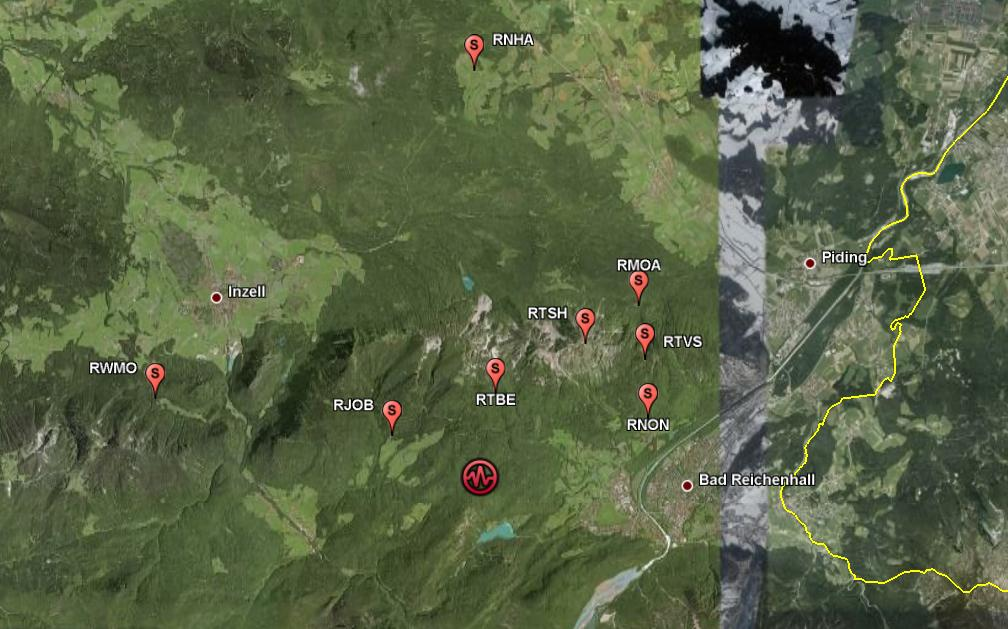
\includegraphics[width=0.8\textwidth]{rh.jpg}
\\[-1ex]{\tiny [http://earth.google.com]}
\end{center}
\vspace*{1.2em}

\exercise{Estimate Local Magnitude}\\
Use the file \verb#RJOB_WA_CUT.MSEED# to read \verb#MiniSEED# waveform data of
the earthquake. These data have already been simulated to displacement on a
Wood-Anderson seismometer (m) and trimmed to the right time span. Estimate the
zero-to-peak amplitude $amp_{zp}$ as half the mean of the maximum minus minimum
amplitude on North and East components in the given short time window (Note
that this is in general not a valid estimation). Estimate the local magnitude
$M_l$ using a hypocentral distance of $d_{hypo}=7.1$ (km) given the following
formula (\verb#Bakun&Joyner, BSSA, 1984#; mathematical functions are available
in the \verb#math# module):

\[
M_l = \log_{10}\left(amp_{zp} * 1000\mathrm{\frac{mm}{m}}\right) +
      \log_{10}\left(\frac{d_{hypo}}{100\mathrm{km}}\right) +
      0.00301 * (d_{hypo} - 100\mathrm{km}) + 3
\]
\vspace*{3.0em}

\exercise{Simulate Wood-Anderson Seismometer}\\
Use the file \verb#RJOB.MSEED# to read the original \verb#MiniSEED# waveform
data. Set up two dictionaries containing the response information of both
the original instrument (an \verb#STS-2#) and the Wood-Anderson seismometer in
poles-and-zeros (\verb#PAZ#) formulation. Each \verb#PAZ# dictionary needs to
contain \verb#sensitivity# (overall sensitivity of seismometer/digitizer
combination), \verb#gain# (normalization factor), \verb#poles# and
\verb#zeros#. After the instrument simulation, trim the waveform to a short
time window around the origin time (\verb#2008-04-17T16:00:32Z#) and calculate
$M_l$ like in exc. 1. Use the following values for the \verb#PAZ# dictionaries:
{\footnotesize
\begin{verbatim}
    STS-2  'sensitivity': 2516778600.0
           'gain': 60077000.0
           'poles': [-0.037004+0.037016j, -0.037004-0.037016j, -251.33+0j,
                     -131.04-467.29j, -131.04+467.29j]
           'zeros': [0j, 0j]
    Wood-Anderson  'gain': 1
                   'sensitivity': 2800
                   'poles': [-6.2832-4.7124j, -6.2832+4.7124j]
                   'zeros': [0j]
\end{verbatim}
}
\vspace*{1.5em}

\exercise{Compare to EMSC Catalog}\\
Fetch a list of events from NERIES/EMSC for the time of the earthquake in the
Hochstaufen region (47.75 N, 12.85 E) using the \verb#Client# provided in
\verb#obspy.neries#. Check if the estimated magnitudes so far roughly match the
magnitude information in the catalog.
\vspace*{2.5em}

\exercise{Fetch Data from WebDC}\\
Modify exc. 2 to fetch the waveform data via ArcLink from WebDC using
\verb#obspy.arclink#. Use keyword argument \verb#getPAZ=True# to fetch response
information along with the waveform. The \verb#PAZ# information will get
attached to the \verb#Stats# object of all traces in the returned \verb#Stream#
object during the waveform request automatically. During instrument simulation
use keyword argument \verb#paz_remove='self'# to use the attached \verb#PAZ#
information fetched from WebDC. Calculate $M_l$ like in exc. 2.
\vspace*{2.5em}

\exercise{Compute Hypocentral Distance}\\
Modify exc. 4 to fetch coordinate information for station \verb#RJOB# along
with the waveform (in a similar manner to the \verb#PAZ#). Use exc. 3 to fetch
the event information from NERIES/EMSC. Use the catalog origin time (stored as
\verb#datetime# in the event dictionary) during the data request from WebDC
instead of the previously hard-coded value. Also calculate the hypocentral
distance dynamically. Use function \verb#utlGeoKm# from module
\verb#obspy.signal# to compute horizontal distances from geographic
coordinates. Calculate $M_l$ like in exc. 4.
\vspace*{2.5em}

\exercise{Determine Event Onset Using a Triggering Algorithm}\\
Read waveform data from file \verb#RJOB.MSEED# and run a recursive STA/LTA
trigger on the Z component of the data. Compute the approximate event onset
time from \verb#starttime# and \verb#sampling_rate# of the trace and from the
position of the maximum in the triggered data (see built-in methods of
\verb#numpy.ndarray# objects: \verb#http://docs.scipy.org#
\verb#/doc/numpy/reference# \verb#/generated/numpy.ndarray.html#). Store this
time in an \verb#UTCDateTime# object.
\vspace*{2.5em}
\newpage
\vspace*{2.5em}

\exercise{Use Trigger Time for Time Window Selection}\\
Modify exc. 5 to use a dynamically determined trigger time like in exc. 6 for
the trimming operations on the waveform data. Calculate $M_l$ like in exc. 5.
\vspace*{3.0em}

\exercise{Estimate Magnitudes for a List of Stations}\\
Modify exc. 7 and use a list of stations (e.g. \verb#RJOB#, \verb#RMOA# and
\verb#RNON#) instead of just a single one. Loop over this list and estimate the
magnitude for each station individually.
\vspace*{3.0em}

\exercise{Fetch List of Available Stations from WebDC}\\
Fetch a list of available stations in network \verb#BW# for the time around the
earthquake\\ (\verb#2008-04-17T16:00:32Z#) via ArcLink from WebDC. Print the
station code for every station in the list.
\vspace*{3.0em}

\exercise{Estimate Magnitudes at All Available Stations}\\
Modify exc. 8 to fetch a list of stations like in exc. 9. Loop over this list,
fetch the data and estimate the magnitude for each of the stations like
before.\\
Note: Not all reported stations really have waveforms for that time span. You
can put the \verb#getWaveform(..)# call inside a \verb#try/except# statement
(see Python API) like this to handle the error and avoid the program execution
being interrupted:
{\footnotesize
\begin{verbatim}
            try:
                client.getWaveform(..., station=sta, ...)
            except:
                print "problem with station:", sta
                continue
\end{verbatim}
}
\vspace*{2.0em}

\exercise{Try Program with Events in Vogtland Swarm Region}\\
By now, the program is rather flexible. We can now simply switch to a
completely different set of events. Modify exc. 10 and change the event request
from EMSC to use events in the Vogtland swarm area (roughly 50.2 N, 12.2 E) at
the north-eastern Bavarian border. There are two magnitude 4+ events in the
EMSC catalog in 2008 that we can use, for instance. Either use one single event
like before or add an additional \verb#for# loop going through all requested
events.
\vspace*{3.0em}

\exercise{Organize Magnitude Estimation in New Python Module}\\
At the end we can clean up the program we wrote by extracting the magnitude
estimation steps in a separate, new Python module. Make a new Python file
\verb#mess_exercise_12_module.py# with a function called
\verb#def estimate_magnitude(...)#. This function should expect four arguments:
\begin{inparaenum}[\itshape a\upshape)] \item a \verb#Stream# object containing
Z, N and E traces with attached \verb#PAZ# and coordinate information, \item
the longitude of the event, \item the latitude of the event and \item the depth
of the event. \end{inparaenum} Move the signal processing steps to this new
module and modify exc. 11 to import and use the function
\verb#estimate_magnitude(...)#.
\vspace*{3.0em}

\end{document}
